\documentclass{article}

\usepackage[utf8]{inputenc}
\usepackage[T1]{fontenc}
\usepackage{lipsum}
\usepackage{graphicx}
\usepackage{amsmath}
\usepackage[margin=1in]{geometry}
\usepackage{titlesec}
\usepackage{enumitem}

\titleformat{\section} 
{\LARGE\bfseries}{\thesection}{1em}{}

\titleformat{\subsection} 
{\Large\bfseries}{\thesection}{1em}{}

\begin{document}

\pagestyle{empty}

\section*{Progettazione di basi di dati} 
\large

Fino ad ora si è visto come \textbf{implementare} una base di dati in SQL, partendo da uno schema relazionale già definito. Per realizzare un sistema informativo \textbf{da zero} bisogna definire una prima fase di \textbf{progettazione}, altrimenti partire direttamente con l'implementazione delle tabelle SQL diventerebbe complesso se non impossibile.\\
Sono presenti diversi problemi nella fase di progettazione di un sistema informativo:
\begin{enumerate}[leftmargin=1cm]
    \itemsep0em
    \item \textbf{Dimensionamento del problema}: un database di un sistema informativo di medie dimensioni può contenere decine di tabelle
    \item \textbf{Analisi dei requisiti}: comprendere le specifiche del sistema, i dati d'interesse del modello e capire quali sono le operazioni sui dati da gestire
    \item \textbf{Traduzione nel modello logico (relazionale)}: una volta chiariti i dubbi sul cosa si deve realizzare, si passa da una \textbf{specifica informale} ad uno \textbf{schema logico}. Senza una buona progettazione, possono emergere \textbf{anomalie ed errori} in questa fase di traduzione
\end{enumerate}
Esistono quindi diverse \textbf{metodologie} per progettare una \textit{buona} base di dati \textbf{a partire dai suoi requisiti}. In generale, la progettazione è solo uno dei componenti del \textbf{ciclo di vita} di un sistema informativo.
\begin{center}
    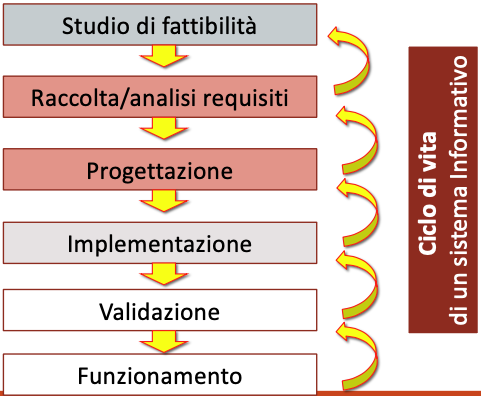
\includegraphics[width=0.38\textwidth]{foto 1.png}
\end{center}
Precedentemente c'è stato un focus sul modulo dell'\textbf{implementazione}, ora si ci soffermerà sui moduli di \textbf{raccolta/analisi dei requisiti} e \textbf{progettazione}.\vspace*{14pt}\\
Si osservi ora il seguente schema:
\begin{center}
    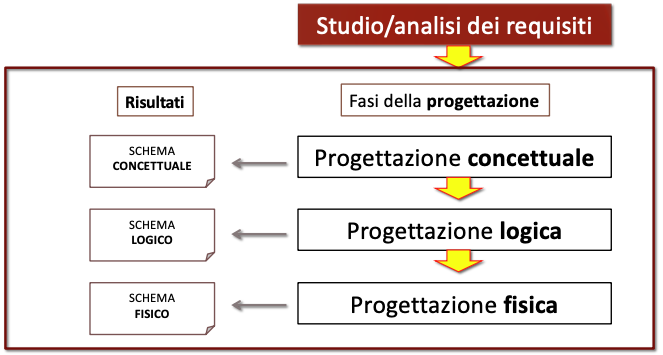
\includegraphics[width=0.65\textwidth]{foto 2.png}
\end{center}
\textit{Studio/analisi dei requisiti}\\
In questa prima fase ci si sofferma sulla specifica dei requisiti e delle operazioni sui dati. Viene letta una traccia o si parla direttamente con un cliente per definire le diverse caratteristiche della base di dati.\vspace*{14pt}\\
\textit{Fasi della progettazione}\\
Durante il corse ci si baserà su una \textbf{metodologia} di progettazione di basi di dati basata su 3 fasi distinte:
\begin{center}
    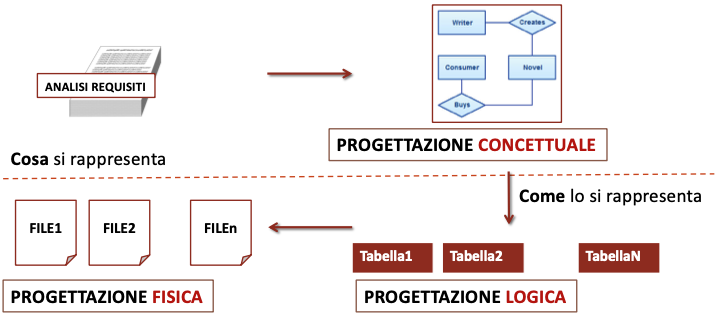
\includegraphics[width=0.65\textwidth]{foto 3.png}
\end{center}
Ogni fase della progettazione produce una \textbf{rappresentazione} della base di dati attraverso uno \textbf{schema}.\vspace*{14pt}\\
\textit{Progettazione concettuale}\\
In questa fase ci si focalizza sul \textbf{contenuto informativo} dei dati ad alto livello di astrazione, senza focalizzarsi sull'implementazione nel modello logico di riferimento. In output si produce un \textbf{modello concettuale} indipendente dallo schema logico e dal DBMS in uso. La progettazione concettuale permette di creare un'\textbf{astrazione completa} dei dati da rappresentare, di capire le \textbf{dipendenze concettuali} tra i dati del modello e di fornire una \textbf{documentazione} della base di dati.\\
Esistono diverse \textbf{alternative} per produrre uno schema concettuale, come il \textbf{modello entità-relazione (ER)} e l'\textbf{Unified Modeling Language (UML)}.\vspace*{14pt}\\
\textit{Progettazione logica}\\
In questa fase si rappresenta la base di dati nello \textbf{schema logico} del DBMS (nel corso si parlerà sempre del modello relazionale). La \textbf{progettazione logica} comprende sia la \textbf{traduzione} dello schema concettuale, sia l'\textbf{ottimizzazione} dello schema logico ottenuto dalla traduzione. Infatti, una volta ottenuto lo schema logico, è necessario analizzare la \textbf{qualità} del prodotto finale. Questa analisi viene effettuata tramite due step:
\begin{itemize}[label={-}, leftmargin=1cm]
    \itemsep0em
    \item \textbf{Rimozione delle ridondanze (normalizzazione)}
    \item \textbf{Analisi delle prestazioni}
\end{itemize}
\textit{Progettazione fisica}\\
In questa fase si descrivono le \textbf{strutture} per la memorizzazione dei dati su memoria secondaria, e l'accesso efficiente ai dati. Alcune strutture utilizzabili sono la \textbf{sequenziale}, \textbf{ad accesso calcolato (hash)} e \textbf{ad albero}.
\end{document}